\chapter{Dynamic point load on elastic halfspace}


% ----------------------------------------------------------------------------------------------
\section{Introduction}
% ----------------------------------------------------------------------------------------------
This benchmark compares the STEM numerical solution against the analytical solution
for a dynamic point load applied to the surface of an elastic half-space.

The analytical solution was derived by Pekeris and is detailed in~\cite{Verruijt_2010}.
The analytical solution provides closed-form expressions for the vertical displacement along the surface of the
half-space, enabling a direct time-history comparison against the numerical model.


% ----------------------------------------------------------------------------------------------
\section{Model Description}
% ----------------------------------------------------------------------------------------------

% ..............................................................................................
\subsection{Geometry, Mesh and Loading}
% ..............................................................................................
The point load was modelled in a three-dimensional domain representing an elastic half-space.
An overview of the geometry for the numerical analysis is shown in Figure~\ref{fig:3D_scheme}.
The soil has a width, length and depth of \qty{5}{\meter} and is subjected to a compressive pulse load, $F(t)$,
which is suddenly applied at the top edge:

\begin{equation}
    F(t) =
     \begin{cases}
    0, & \text{if } t<0\\
    \qty{-1000}{\kilo\newton}, & \text{if } t>0\\
    \end{cases}
\end{equation}


\begin{figure}
    \centering
    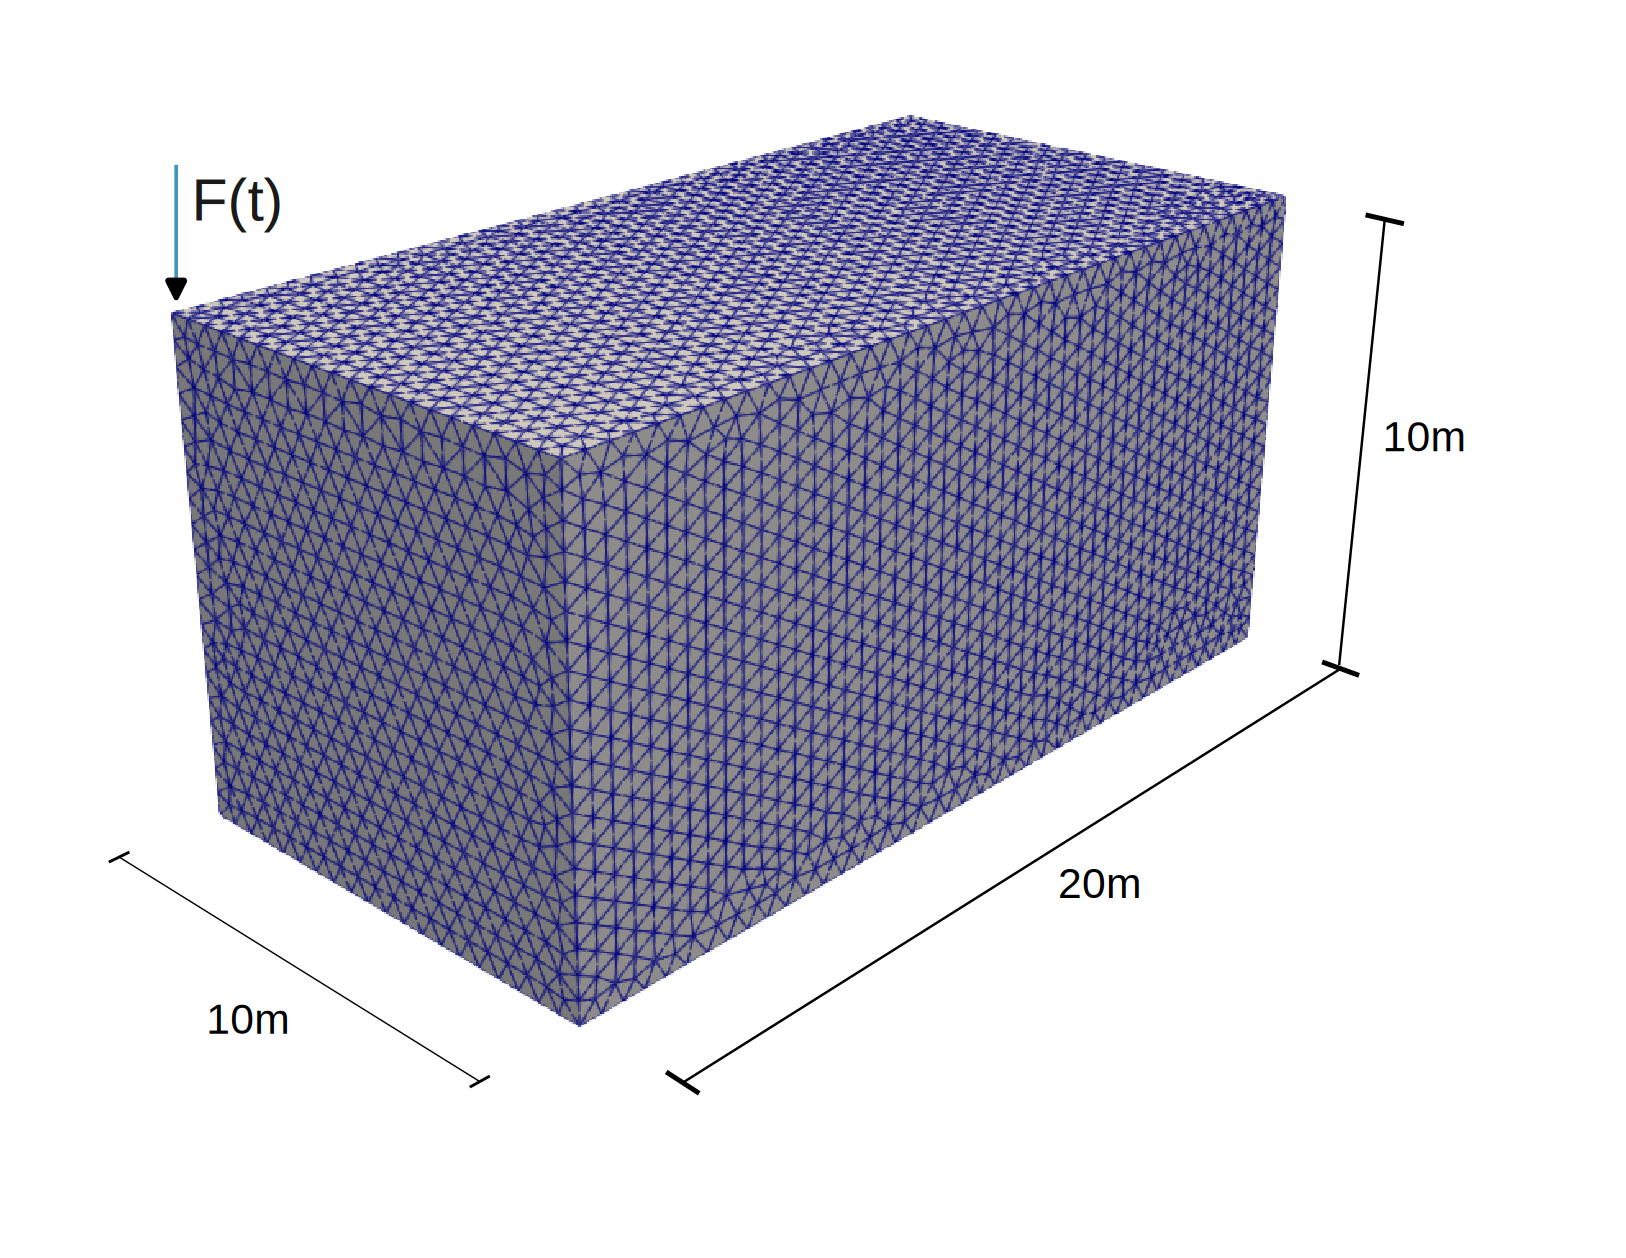
\includegraphics[width=0.75\textwidth]{pekeris/mesh.pdf}
    \caption{Geometry, mesh and loading conditions for the three-dimensional wave propagation problem.}
    \label{fig:3D_scheme}
\end{figure}

The soil is discretised in high-order tetrahedral elements with size \qty{0.15}{\meter}.
In total the model comprises 596~493~elements.

The nodes at the sides of the soil have absorbing boundaries at the free ends, and with fixed boundary conditions
on the perpendicular plane along the axis of symmetry.
At the bottom the soil is assumed to be fixed, simulating the existence of the top of bedrock that has a
significantly larger stiffness than the soil above.

% ..............................................................................................
\subsection{Materials and numerical parameters}
% ..............................................................................................
The soil is modelled as an one-phase continuum with a linear elastic constitutive law, with the
following parameters:

\begin{itemize}[noitemsep,topsep=0pt,parsep=0pt,partopsep=0pt]
    \item Young's modulus: \qty{30}{\mega\pascal},
    \item Poisson ratio: \qty{0.3},
    \item Density: \qty{2000}{\kilogram\per\meter\cubed}.
\end{itemize}

% ----------------------------------------------------------------------------------------------
\section{Results}
% ----------------------------------------------------------------------------------------------
Figure~\ref{fig:pekeris_results} presents the time histories of the vertical displacement for three
nodes. located at 1, 2 and~\qty{3}{\meter} from the load, located along the surface.
The figure compares the STEM results against the analytical solution.
If follows that there is an agreement between both solutions, demonstrating the accuracy of the STEM
for this type of dynamic loading condition.

\begin{figure}[h]
    \centering
    \includegraphics[width=0.8\textwidth]{pekeris/time_history.pdf}
    \caption{Comparison of the vertical displacement time histories at surface nodes located at:
     (a) \qty{1}{\meter}, (b) \qty{2}{\meter} and (c) \qty{3}{\meter} from the load.}
    \label{fig:pekeris_results}
\end{figure}
